\documentclass[bachelor]{thesis-uestc}
\usepackage{indentfirst}
\usepackage{amssymb, amsmath}
\usepackage{graphicx, subfigure}
\usepackage{algorithm, algorithmic, float}
% 没有使用thesis-uestc的算法模板, 需将thesis-uestc中的相关内容注释掉, 避免冲突
\usepackage{listings}
\usepackage{fancyhdr}
\usepackage{booktabs}

% ----------------------------------------- Document -----------------------------------------

\begin{document}

% ----------------------------------------- 目录 -----------------------------------------
\thesistableofcontents

% ----------------------------------------- 正文 -----------------------------------------
\thesischapterexordium % 需求分析

\section{总体要求}
\begin{itemize}
	\item 存储一张表,然后能对该表进行查询、添加等操作。上述功能以API的形式提供给应用使用。
\end{itemize}

\begin{figure}[htbp]
	\centering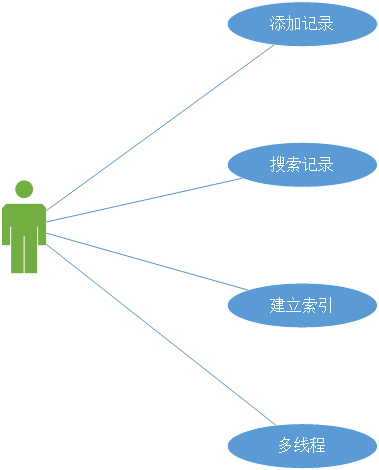
\includegraphics[height=6cm]{images/use_case.png}
	\caption{用例图}
	\label{fig:use_case}
\end{figure}

\section{存储要求}
\begin{itemize}
	\item 存储一张表,然后能对该表进行查询、添加等操作。上述功能以API的形式提供给应用使用。
	\item 该表有100个属性,每个属性都是int64\_t类型;
	\item 需要支持的最大行数为1百万行。
\end{itemize}

\section{添加要求}
\begin{itemize}
	\item 提供API函数,实现向表格添加一行的功能(添加到表格的末尾)。
\end{itemize}

\section{搜索要求}
\begin{itemize}
	\item 提供API函数,实现对表格的某一个属性进行范围查找的功能。例如:查找在属性A上,大于等于50,小于等于100的所有行
	\item 用户可以指定在哪一个属性上进行搜索;
	\item 当搜索结果包含的行数过多时,可以只返回一小部分,如10行等。
\end{itemize}

\section{索引要求}
\begin{itemize}
	\item 提供API函数,为表格的某一个属性建立索引结构,以实现快速搜索;
	\item 自行选择使用哪种数据结构,建立索引结构,比如B+树等;
	\item 建立的索引结构,需要保存到一个文件中(索引文件);下次重启应用程序,并执行搜索任务时,应先检查是否已为相应属性建立了索引结构;
	\item 即,搜索功能实现时,需要查找是否有索引文件存在,若有,则使用该文件加速搜索。	
\end{itemize}

\section{并发要求}
\begin{itemize}
	\item 应用程序可以以多线程的方式,使用我们提供的上述API;
	\item 要保证多线程环境下,表、索引结构、索引文件的一致性。
\end{itemize}

\chapter{总体设计}
\section{整个程序的架构}
存储引擎维护三个文件:table\_file,index\_file,manifest\_file。其中,table\_file负责用户添加数据的持久化;index\_file负责索引结构的持久化;manifest\_file负责存储元数据,以便重启程序后进行恢复。\par
用户在使用该引擎时可以以多线程方式向表中添加数据和查询数据,但建立索引时必须以单线程方式,因为索引结构属于全局结构,即整个表只有一个索引结构。如果以多线程方式建立索引就会存在一个问题:如果线程A建立了索引,那么这个索引结构只是针对线程A所添加的数据而建立的;如果线程B被调度,并且尝试建立索引,那么线程A建立的索引就会需要合并上线程B添加的数据所对应的索引。当多个线程并发地添加数据并尝试建立索引时,索引结构就会被频繁修改,造成效率的降低。基于上述考虑,该存储引擎在设计时只允许以单线程的方式建立索引,如果多线程并发添加数据,那么必须等到所有线程结束后再给表中的属性建立索引。\par
另外,索引结构只有一个,也就是说同一时刻只存在表中的某一个属性的索引。当尝试为别的属性建立索引时,旧的索引结构就会被删除。\par
存储引擎在开发时进行了跨平台处理,支持Linux和Windows平台。

\section{关键流程分析}
\subsection{添加数据}
添加数据的流程图如图\ref{fig:append}所示。因为添加数据要实现多线程安全,所以需要先获得互斥锁,然后判断table\_file文件是否有效、用户输入是否有效等,检查成功后就可以将编码后的数据使用追加写的方式写入table\_file。

\begin{figure}[htbp]
	\centering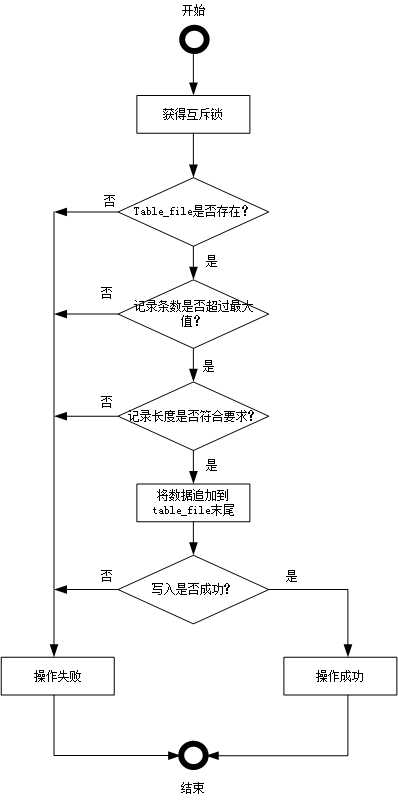
\includegraphics[height=10cm]{images/append.png}
	\caption{添加数据}
	\label{fig:append}
\end{figure}

\subsection{建立索引}
建立索引的流程图如图\ref{fig:build_index}所示。为标号为attr\_id所对应的属性列建立索引时,如果用户没有显式告知存储引擎,添加数据已经结束,那么程序就主动结束数据的添加,关闭可写的table\_file文件,并重新以只读方式打开table\_file。然后从table\_file读入需要建立索引的属性列的全部数据,构造一个IndexEntry结构的线性表(IndexEntry结构包含两个数据,一个是表中的数据,一个是该数据所在的行号),将其排序后写入index\_file。写入成功后重新打开一个只读的index\_file以便后续的查询操作所使用。

\begin{figure}[htbp]
	\centering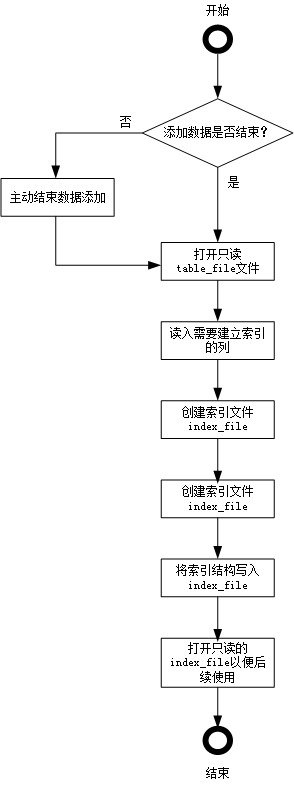
\includegraphics[height=10cm]{images/build_index.png}
	\caption{建立索引}
	\label{fig:build_index}
\end{figure}

\subsection{查询数据}
查询数据时用户需要指定一个属性,以及在该属性上查询的范围。如果索引文件不存在就直接读取表数据文件进行顺序查找,每次读取一行数据(100个属性),判断给定属性的值是否在用户指定的查询区间内,如果是,就说明将该行数据添加到查询结果中。如果索引文件存在,就可以加速查询。因为索引结构实则是一个KV结构的数组,Key就是相应属性上的值,Value就是该属性值所属的行号,根据行号可以实现表数据文件table\_file的随机读取。查询数据的具体流程如图\ref{fig:lookup}所示。

\begin{figure}[htbp]
	\centering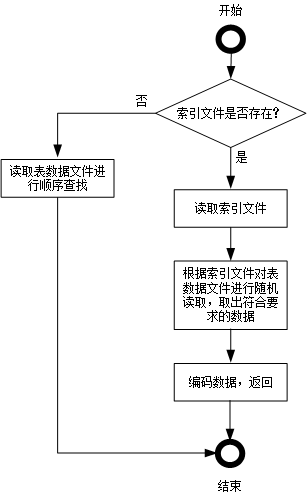
\includegraphics[height=10cm]{images/lookup.png}
	\caption{查询数据}
	\label{fig:lookup}
\end{figure}

\chapter{详细设计与实现}
\section{文件I/O与跨平台}
存储引擎只支持两种类型的文件:写入方式只能是追加写的可写文件WritableFile,支持随机读的只读文件RandomAccessFile。这两个文件抽象类对Linux和Windows都有具体的实现,跨平台的核心就是底层的文件操作接口。相关类图如图\ref{fig:randonaccessfile}和图\ref{fig:writablefile}所示。

\begin{figure}[htbp]
	\centering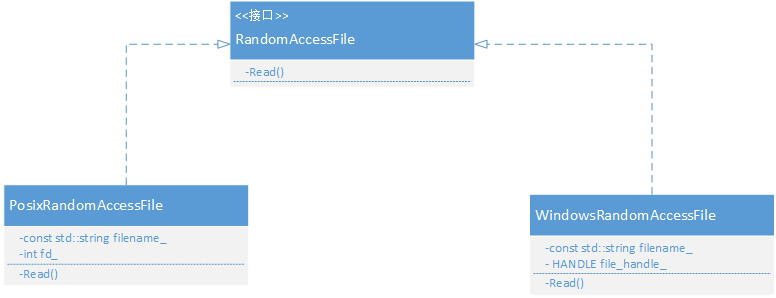
\includegraphics[height=3.5cm]{images/randomaccessfile.png}
	\caption{RandomAccessFile类图}
	\label{fig:randonaccessfile}
\end{figure}

\begin{figure}[htbp]
	\centering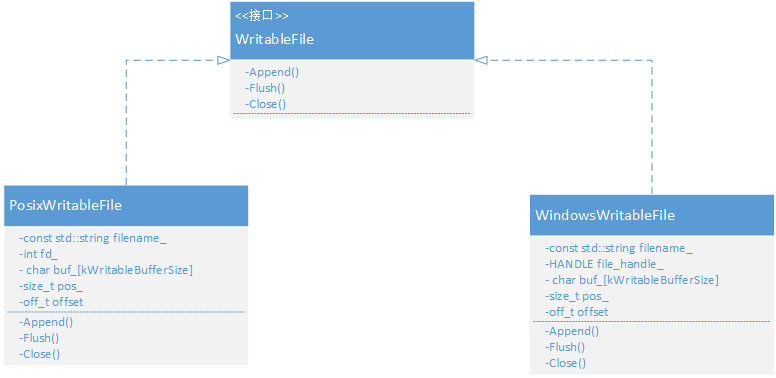
\includegraphics[height=3.5cm]{images/writablefile.png}
	\caption{WritableFile类图}
	\label{fig:writablefile}
\end{figure}

抽象基类RandomAccessFile/WritableFile的子类实例分别由抽象基类Env的子类WindowsEnv/PosixEnv实例创建,使用工厂方法模式。Env及其子类的类图如图所示。

\begin{figure}[htbp]
	\centering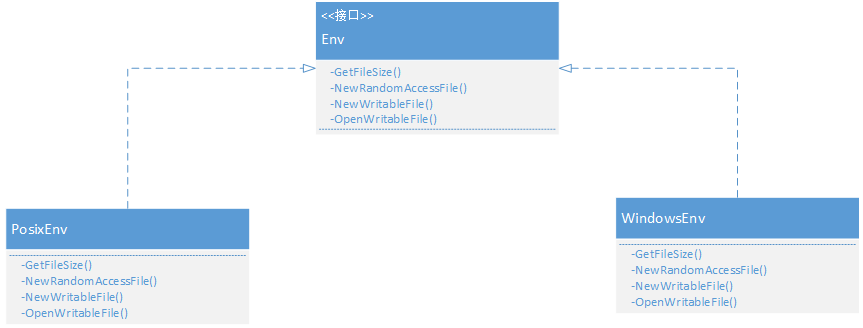
\includegraphics[height=3.5cm]{images/env.png}
	\caption{Env类图}
	\label{fig:env}
\end{figure}

\subsection{文件I/O具体实现}
\subsubsection{文件随机读}
Linux平台上,PosixRandomAccessFile::Read()使用pread()系统调用根据给定的偏移量随机读;Windows平台上,WindowsRandomAccessFile::Read()使用ReadFile()和参数OVERLAPPED实现随机读。

\subsubsection{文件追加写}
调用WritableFile::Append()写文件时先将数据写入内存缓冲,当缓冲区满后再Flush到磁盘,以此减少磁盘I/O次数提高效率。

\subsection{Env工厂方法具体实现}
抽象基类Env提供了4个接口:GetFileSize()获取文件大小;NewRandomAccessFile()创建一个RandomAccessFile子类实例;NewWritableFile()和OpenWritableFile()都是创建一个WritableFile子类实例,是不过New*会新建一个文件;Open*打开一个已存在的文件,并将文件指针移到文件末尾。\par
Linux平台上PosixEnv::GetFileSize()使用stat()系统调用,Windows平台上WindowsEnv::GetFileSize()先使用CreateFile()打开文件,获得文件句柄,再使用GetFileSize()系统调用获得文件大小,最后CloseHandle()关闭文件句柄。\par
Linux平台上PosixEnv::NewRandomAccessFile()/NewWritableFile()使用open()系统调用打开文件,Windows平台上WindowsEnv::NewRandomAccessFile()/NewWritableFile()使用CreateFile()系统调用打开文件。这里需要注意,Linux的open()打开的文件默认是非阻塞的,即文件打开到关闭期间,可以调用open()再次打开之;但是Windows需要给CreateFile()指定FILE\_SHARE\_READ或FILE\_SHARE\_WRITE显式地创建为非阻塞模式,否则在关闭文件前无法再次打开之。

\chapter{测试}


\end{document}
